% Source: outputs/run_20261106_193109_gate_provenance (notes §84, results T107).
\subsection{Where the gates come from, and whether they favour \vkid{}}
\label{app:gateprov}

\vkid{} and the gates that admit it come from one project, so the gates need
evidence that they were not shaped around it. We give three kinds: each gate's
prior use, when each threshold was set, and the verdicts of
Table~\ref{tab:headtohead} under alternative thresholds.

\paragraph{Prior use.} Table~\ref{tab:gateprov} maps each gate to earlier work
that states the same criterion. Ordering under graded corruption is the test
FID was introduced with \citep{heusel2017fid}, repeated for KID
\citep{binkowski2018kid} and made a rank-correlation criterion for graph
metrics \citep{obray2022graphmetrics,thompson2022evaluation}. Invariance to
quality-preserving transforms is a stated desideratum
\citep{borji2019prosandcons,borji2022newdevelopments}, and FID's violations of
it are documented \citep{kynkaanniemi2023imagenet,parmar2022aliased}. A metric
that cannot recognise two samples of one distribution fails the test
\citet{naeem2020prdc} apply to precision and recall, and sample-size bias is
the defect \citet{binkowski2018kid}, \citet{chong2020unbiasedfid} and
\citet{jayasumana2024cmmd} identify in FID. The memorization gates follow the
held-out-referenced data-copying test of \citet{meehan2020datacopying}, and the
within-set twin gate follows the approximate-copy diversity test of
\citet{jiralerspong2023fld}. Text-metric checklists apply the same
directional and invariance tests \citep{ribeiro2020checklist,sai2021perturbation}.
What we change is the use: a failing metric is withheld from ranking rather
than reported with a caveat. \citet{obray2022graphmetrics} use graded perturbations
to select metric hyperparameters, never to disqualify a metric, and without an
invariance or sample-size test; \citet{borji2019prosandcons} list the desiderata
without running them as a gate. The one prior meta-evaluation of metrics in this
domain, \citet{herve2021pcgmetrics}, correlates eighteen procedural-content metrics
with GDMC jury scores, the route a human-validated version of this suite would take.

\begin{table}[h]
\centering
\small
\setlength{\tabcolsep}{3pt}
\begin{tabular}{lp{0.62\linewidth}}
\toprule
gate & prior statement of the criterion \\
\midrule
G1, G2 ordering & \citet{heusel2017fid,binkowski2018kid,xu2018empirical,obray2022graphmetrics,thompson2022evaluation,jayasumana2024cmmd,jiralerspong2023fld} \\
G6 invariance & \citet{borji2019prosandcons,borji2022newdevelopments,kynkaanniemi2023imagenet,parmar2022aliased,ribeiro2020checklist} \\
G7 self-consistency & \citet{naeem2020prdc,binkowski2018kid,lopezpaz2017c2st,yang2019pointflow} \\
G8 $n$-stability & \citet{binkowski2018kid,chong2020unbiasedfid,jayasumana2024cmmd,jiralerspong2023fld,thompson2022evaluation} \\
memorization & \citet{meehan2020datacopying,alaa2022faithful,jiralerspong2023fld,stein2023exposing,somepalli2023replication} \\
diversity, twins & \citet{xu2018empirical,naeem2020prdc,jiralerspong2023fld} \\
\bottomrule
\end{tabular}
\caption{\textbf{Each gate restates a published criterion.}}
\label{tab:gateprov}
\end{table}

\paragraph{When the thresholds were set.} The ordering, invariance, self-consistency and $n$-stability thresholds were committed and validated on render
metrics four weeks before the first voxel-descriptor metric existed, and the gate code,
with the $77$-dimensional descriptor, has been unchanged for $58$ days before the
head-to-head of Sec.~\ref{app:headtohead} ran. The only later change to the gates is the
pair of denominator corrections of Sec.~\ref{app:defects}, which apply to every metric;
the twin gate reuses the duplicate gate's rule.

\paragraph{Verdicts under other thresholds.} We recompute every gate of
Table~\ref{tab:headtohead} from the stored scores and, for \vkid{}, occupancy KID
and the six IoU rows, from a rerun that reproduces the table to $2\times10^{-6}$
and also records each null mean and drift. Each threshold moves over a range
around its value: ordering tolerance from $-1$ (each step must rise by one
floor) to $+2$ (a step may fall by two), the invariance bar from $0.5$ to $5$
floors, and the self-consistency and $n$-stability bars from $1$ to $5$.
\begin{itemize}
\item At every ordering tolerance $\le 0$ and every invariance bar, with the
  other two bars at their values, \vkid{} is the only row that passes
  (Fig.~\ref{fig:gatesweep}).
\item \vkid{} passes in all $360$ of the $480$ joint settings with a
  self-consistency bar of at least $2$ floors. A bar of $1$ floor rejects every
  row, \vkid{} included, as a single draw lies within one floor of its mean only
  about two thirds of the time.
\item Its margins are wide: the smallest ordering step is $7.5$ floors,
  invariance holds exactly, the self-consistency deviation is $1.2$ floors and the
  drift is $0.4$ standard errors.
\item The rows a looser threshold admits are those whose failure is a tie
  rather than an inversion. Allowing a step to fall by half a floor admits
  1-NNA on IoU and EMD, which separate \solidify{} by $2.7$ and $1.6$ floors;
  adding an invariance bar of $2$ floors admits occupancy KID ($48.4$). No
  threshold admits an encoder as a geometry metric, since \matshuffle{} and
  \monochrome{} move them by $63$ to $106$ floors, nor IoU nearest-neighbour MMD,
  whose $n$-drift is $34$ to $36$ standard errors.
\end{itemize}
The same holds for disqualification. Across novelty bars of $2$, $3$ and $5$
spreads and floors of half, one and two times their values, both positive
controls, Dream-Cubed and the hollow-box baseline are disqualified in all nine
settings. Only the loosest corner readmits an arm, the gabled-house baseline, and tightening to $2$ spreads first
disqualifies our own autoregressive arms on DINO nearest-neighbour percentile.

\begin{figure}[h]
\centering
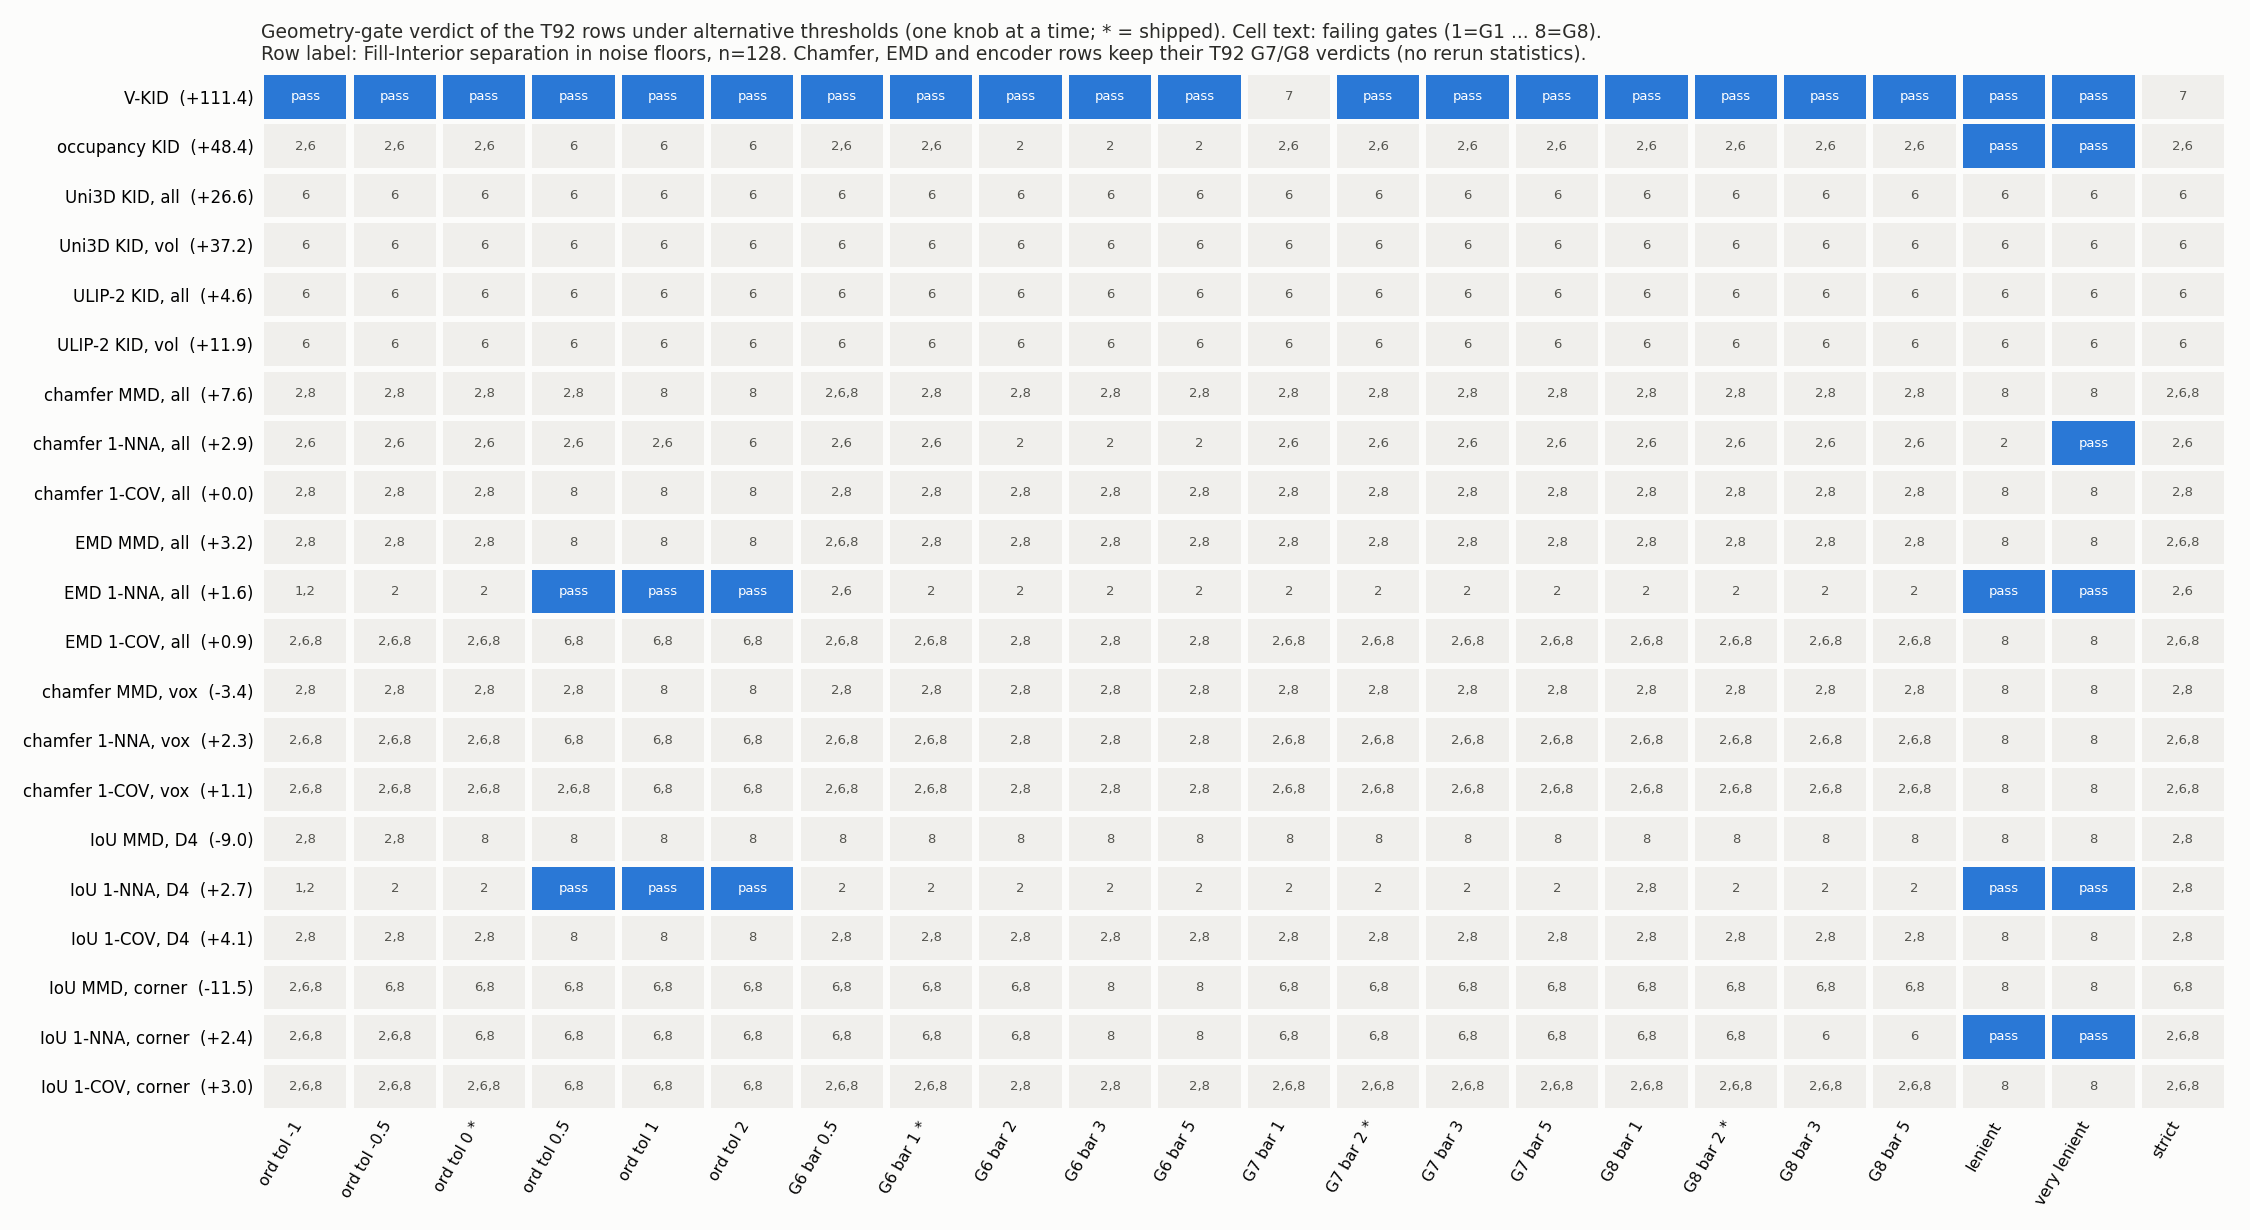
\includegraphics[width=\linewidth]{figures/gate_sweep.png}
\caption{\textbf{Gate verdicts under alternative thresholds.} Rows of
Table~\ref{tab:headtohead} with their \solidify{} separation; columns move one
threshold at a time ($*$ marks the value used) or all four together. Blue:
passes every gate on the geometry rungs. Text: the gates that fail.}
\label{fig:gatesweep}
\end{figure}
